%%%%%%%%%%%%%%%%%%%%%%%%%%%%%%%%%%%%%%%%%
% Lachaise Assignment
% LaTeX Template
% Version 1.0 (26/6/2018)
%
% This template originates from:
% http://www.LaTeXTemplates.com
%
% Authors:
% Marion Lachaise & François Févotte
% Vel (vel@LaTeXTemplates.com)
%
% License:
% CC BY-NC-SA 3.0 (http://creativecommons.org/licenses/by-nc-sa/3.0/)
% 
%%%%%%%%%%%%%%%%%%%%%%%%%%%%%%%%%%%%%%%%%

%----------------------------------------------------------------------------------------
%	PACKAGES AND OTHER DOCUMENT CONFIGURATIONS
%----------------------------------------------------------------------------------------

\documentclass[utf-8]{article}
\usepackage[UTF8, scheme = plain]{ctex}
\usepackage{subfigure}
\usepackage{float}

%%%%%%%%%%%%%%%%%%%%%%%%%%%%%%%%%%%%%%%%%
% Lachaise Assignment
% Structure Specification File
% Version 1.0 (26/6/2018)
%
% This template originates from:
% http://www.LaTeXTemplates.com
%
% Authors:
% Marion Lachaise & François Févotte
% Vel (vel@LaTeXTemplates.com)
%
% License:
% CC BY-NC-SA 3.0 (http://creativecommons.org/licenses/by-nc-sa/3.0/)
% 
%%%%%%%%%%%%%%%%%%%%%%%%%%%%%%%%%%%%%%%%%

%----------------------------------------------------------------------------------------
%	PACKAGES AND OTHER DOCUMENT CONFIGURATIONS
%----------------------------------------------------------------------------------------

\usepackage{amsmath,amsfonts,stmaryrd,amssymb} % Math packages

\usepackage{enumerate} % Custom item numbers for enumerations

\usepackage[ruled]{algorithm2e} % Algorithms

\usepackage[framemethod=tikz]{mdframed} % Allows defining custom boxed/framed environments

% \usepackage{listings} % File listings, with syntax highlighting
% \lstset{
% 	basicstyle=\ttfamily, % Typeset listings in monospace font
% }
\usepackage{listings}
\usepackage{ctex}

% 用来设置附录中代码的样式

% \lstset{
%     basicstyle          =   \sffamily,          % 基本代码风格
%     keywordstyle        =   \bfseries,          % 关键字风格
%     commentstyle        =   \rmfamily\itshape,  % 注释的风格,斜体
%     stringstyle         =   \ttfamily,  % 字符串风格
%     flexiblecolumns,                % 别问为什么,加上这个
%     numbers             =   left,   % 行号的位置在左边
%     showspaces          =   false,  % 是否显示空格,显示了有点乱,所以不现实了
%     % numberstyle         =   \zihao{-5}\ttfamily,    % 行号的样式,小五号,tt等宽字体
%     showstringspaces    =   false,
%     captionpos          =   t,      % 这段代码的名字所呈现的位置,t指的是top上面
%     frame               =   lrtb,   % 显示边框
% 		%backgroundcolor=\color{red!50!green!50!blue!50},%代码块背景色为浅灰色
% %	rulesepcolor= \color{gray}, %代码块边框颜色
% 	breaklines=true,  %代码过长则换行
% 	% numbers=left, %行号在左侧显示
% 	numberstyle= \small,%行号字体
% 	keywordstyle= \color{blue},%关键字颜色
% 	commentstyle=\color{gray}, %注释颜色
% 	%	frame=shadowbox%用方框框住代码块
% 	frame=single,
% 	escapeinside=``    % 代码包含中文
% }

% \lstdefinestyle{Python}{
%     language        =   Python, % 语言选Python
%     basicstyle      =   \zihao{-5}\ttfamily,
%     numberstyle     =   \zihao{-5}\ttfamily,
%     keywordstyle    =   \color{blue},
%     keywordstyle    =   [2] \color{teal},
%     stringstyle     =   \color{magenta},
%     commentstyle    =   \color{red}\ttfamily,
%     breaklines      =   true,   % 自动换行,建议不要写太长的行
%     columns         =   fixed,  % 如果不加这一句,字间距就不固定,很丑,必须加
%     basewidth       =   0.5em,
% }
\lstdefinestyle{lfonts}{
	basicstyle 	= \footnotesize\ttfamily,
	stringstyle	= \color{purple},
	showstringspaces = false,
	keywordstyle = \color{blue!60!black}\bfseries,
	commentstyle = \color{olive},
}

\lstdefinestyle{lnumbers}{
	numbers		= left,
	numberstyle = \tiny,
	numbersep	= 1em,
	firstnumber = 1,
	stepnumber 	= 1,
}

\lstdefinestyle{llayout}{
	breaklines	= true,
	tabsize		= 4,
	columns		= flexible,
}

\lstdefinestyle{lgeometry}{
	xleftmargin		= 20pt,
	xrightmargin	= 0pt,
	frame			= tb,
	framesep		= \fboxsep,
	framexleftmargin	= 20pt,
}

\lstdefinestyle{lgeneral}{
	style	= lfonts,
	style	= lnumbers,
	style	= llayout,
	style	= lgeometry,
}

\lstdefinestyle{python}{
	language	= {Python},
	style		= lgeneral
}

%----------------------------------------------------------------------------------------
%	DOCUMENT MARGINS
%----------------------------------------------------------------------------------------

\usepackage{geometry} % Required for adjusting page dimensions and margins

\geometry{
	paper=a4paper, % Paper size, change to letterpaper for US letter size
	top=2.5cm, % Top margin
	bottom=3cm, % Bottom margin
	left=2.5cm, % Left margin
	right=2.5cm, % Right margin
	headheight=14pt, % Header height
	footskip=1.5cm, % Space from the bottom margin to the baseline of the footer
	headsep=1.2cm, % Space from the top margin to the baseline of the header
	%showframe, % Uncomment to show how the type block is set on the page
}

\usepackage{indentfirst} 

%----------------------------------------------------------------------------------------
%	FONTS
%----------------------------------------------------------------------------------------

\usepackage[utf8]{inputenc} % Required for inputting international characters
\usepackage[T1]{fontenc} % Output font encoding for international characters

\usepackage{XCharter} % Use the XCharter fonts

%----------------------------------------------------------------------------------------
%	COMMAND LINE ENVIRONMENT
%----------------------------------------------------------------------------------------

% Usage:
% \begin{commandline}
%	\begin{verbatim}
%		$ ls
%		
%		Applications	Desktop	...
%	\end{verbatim}
% \end{commandline}

\mdfdefinestyle{commandline}{
	leftmargin=10pt,
	rightmargin=10pt,
	innerleftmargin=15pt,
	middlelinecolor=black!50!white,
	middlelinewidth=2pt,
	frametitlerule=false,
	backgroundcolor=black!5!white,
	frametitle={Command Line},
	frametitlefont={\normalfont\sffamily\color{white}\hspace{-1em}},
	frametitlebackgroundcolor=black!50!white,
	nobreak,
}

% Define a custom environment for command-line snapshots
\newenvironment{commandline}{
	\medskip
	\begin{mdframed}[style=commandline]
}{
	\end{mdframed}
	\medskip
}

%----------------------------------------------------------------------------------------
%	FILE CONTENTS ENVIRONMENT
%----------------------------------------------------------------------------------------

% Usage:
% \begin{file}[optional filename, defaults to "File"]
%	File contents, for example, with a listings environment
% \end{file}

\mdfdefinestyle{file}{
	innertopmargin=1.6\baselineskip,
	innerbottommargin=0.8\baselineskip,
	topline=false, bottomline=false,
	leftline=false, rightline=false,
	leftmargin=2cm,
	rightmargin=2cm,
	singleextra={%
		\draw[fill=black!10!white](P)++(0,-1.2em)rectangle(P-|O);
		\node[anchor=north west]
		at(P-|O){\ttfamily\mdfilename};
		%
		\def\l{3em}
		\draw(O-|P)++(-\l,0)--++(\l,\l)--(P)--(P-|O)--(O)--cycle;
		\draw(O-|P)++(-\l,0)--++(0,\l)--++(\l,0);
	},
	nobreak,
}

% Define a custom environment for file contents
\newenvironment{file}[1][File]{ % Set the default filename to "File"
	\medskip
	\newcommand{\mdfilename}{#1}
	\begin{mdframed}[style=file]
}{
	\end{mdframed}
	\medskip
}

%----------------------------------------------------------------------------------------
%	NUMBERED QUESTIONS ENVIRONMENT
%----------------------------------------------------------------------------------------

% Usage:
% \begin{question}[optional title]
%	Question contents
% \end{question}

\mdfdefinestyle{question}{
	innertopmargin=1.2\baselineskip,
	innerbottommargin=0.8\baselineskip,
	roundcorner=5pt,
	nobreak,
	singleextra={%
		\draw(P-|O)node[xshift=1em,anchor=west,fill=white,draw,rounded corners=5pt]{%
		Question \theQuestion\questionTitle};
	},
}

\newcounter{Question} % Stores the current question number that gets iterated with each new question

% Define a custom environment for numbered questions
\newenvironment{question}[1][\unskip]{
	\bigskip
	\stepcounter{Question}
	\newcommand{\questionTitle}{~#1}
	\begin{mdframed}[style=question]
}{
	\end{mdframed}
	\medskip
}

%----------------------------------------------------------------------------------------
%	WARNING TEXT ENVIRONMENT
%----------------------------------------------------------------------------------------

% Usage:
% \begin{warn}[optional title, defaults to "Warning:"]
%	Contents
% \end{warn}

\mdfdefinestyle{warning}{
	topline=false, bottomline=false,
	leftline=false, rightline=false,
	nobreak,
	singleextra={%
		\draw(P-|O)++(-0.5em,0)node(tmp1){};
		\draw(P-|O)++(0.5em,0)node(tmp2){};
		\fill[black,rotate around={45:(P-|O)}](tmp1)rectangle(tmp2);
		\node at(P-|O){\color{white}\scriptsize\bf !};
		\draw[very thick](P-|O)++(0,-1em)--(O);%--(O-|P);
	}
}

% Define a custom environment for warning text
\newenvironment{warn}[1][Warning:]{ % Set the default warning to "Warning:"
	\medskip
	\begin{mdframed}[style=warning]
		\noindent{\textbf{#1}}
}{
	\end{mdframed}
}

%----------------------------------------------------------------------------------------
%	INFORMATION ENVIRONMENT
%----------------------------------------------------------------------------------------

% Usage:
% \begin{info}[optional title, defaults to "Info:"]
% 	contents
% 	\end{info}

\mdfdefinestyle{info}{%
	topline=false, bottomline=false,
	leftline=false, rightline=false,
	nobreak,
	singleextra={%
		\fill[black](P-|O)circle[radius=0.4em];
		\node at(P-|O){\color{white}\scriptsize\bf i};
		\draw[very thick](P-|O)++(0,-0.8em)--(O);%--(O-|P);
	}
}

% Define a custom environment for information
\newenvironment{info}[1][Info:]{ % Set the default title to "Info:"
	\medskip
	\begin{mdframed}[style=info]
		\noindent{\textbf{#1}}
}{
	\end{mdframed}
}
 % Include the file specifying the document structure and custom commands

%----------------------------------------------------------------------------------------
%	ASSIGNMENT INFORMATION
%----------------------------------------------------------------------------------------

\title{Machine Learning: Assignment 1} % Title of the assignment

\author{\\黄绵秋 \texttt{19307130142@fudan.edu.cn}} % Author name and email address

\date{19级计算机 --- \today} % University, school and/or department name(s) and a date

%----------------------------------------------------------------------------------------

\begin{document}

\maketitle % Print the title

%----------------------------------------------------------------------------------------
%	INTRODUCTION
%----------------------------------------------------------------------------------------

\section*{Assignment 1} % Unnumbered section

使用KNN算法对iris数据集进行分类,采用交叉验证的方式处理训练数据和测试数据

% Math equation/formula
% \begin{equation}
% 	I = \int_{a}^{b} f(x) \; \text{d}x.
% \end{equation}

% Aliquam arcu turpis, ultrices sed luctus ac, vehicula id metus. Morbi eu feugiat velit, et tempus augue. Proin ac mattis tortor. Donec tincidunt, ante rhoncus luctus semper, arcu lorem lobortis justo, nec convallis ante quam quis lectus. Aenean tincidunt sodales massa, et hendrerit tellus mattis ac. Sed non pretium nibh. Donec cursus maximus luctus. Vivamus lobortis eros et massa porta porttitor.

% \begin{info} % Information block
% 	This is an interesting piece of information, to which the reader should pay special attention. Fusce varius orci ac magna dapibus porttitor. In tempor leo a neque bibendum sollicitudin. Nulla pretium fermentum nisi, eget sodales magna facilisis eu. Praesent aliquet nulla ut bibendum lacinia. Donec vel mauris vulputate, commodo ligula ut, egestas orci. Suspendisse commodo odio sed hendrerit lobortis. Donec finibus eros erat, vel ornare enim mattis et.
% \end{info}

%----------------------------------------------------------------------------------------
%	PROBLEM 1
%----------------------------------------------------------------------------------------

\section{{任务描述}} % Numbered section

%------------------------------------------------

\subsection{使用KNN算法对iris数据集进行分类}

% Numbered question, with subquestions in an enumerate environment
% \begin{question}
% 	Quisque ullamcorper placerat. Cras nibh. Morbi vel justo vitae lacus tincidunt ultrices. Lorem ipsum dolor sit amet, consectetuer adipiscing elit.

% 	% Subquestions numbered with letters
% 	\begin{enumerate}[(a)]
% 		\item Do this.
% 		\item Do that.
% 		\item Do something else.
% 	\end{enumerate}
% \end{question}
	
%------------------------------------------------

\subsection{通过优化和调超参来使准确率进一步提高}
 


% \begin{center}
% 	\begin{minipage}{0.5\linewidth} % Adjust the minipage width to accomodate for the length of algorithm lines
% 		\begin{algorithm}[H]
% 			\KwIn{$(a, b)$, two floating-point numbers}  % Algorithm inputs
% 			\KwResult{$(c, d)$, such that $a+b = c + d$} % Algorithm outputs/results
% 			\medskip
% 			\If{$\vert b\vert > \vert a\vert$}{
% 				exchange $a$ and $b$ \;
% 			}
% 			$c \leftarrow a + b$ \;
% 			$z \leftarrow c - a$ \;
% 			$d \leftarrow b - z$ \;
% 			{\bf return} $(c,d)$ \;
% 			\caption{\texttt{FastTwoSum}} % Algorithm name
% 			\label{alg:fastTwoSum}   % optional label to refer to
% 		\end{algorithm}
% 	\end{minipage}
% \end{center}

% Numbered question, with an optional title
% \begin{question}[\itshape (with optional title)]
% 	In congue risus leo, in gravida enim viverra id. Donec eros mauris, bibendum vel dui at, tempor commodo augue. In vel lobortis lacus. Nam ornare ullamcorper mauris vel molestie. Maecenas vehicula ornare turpis, vitae fringilla orci consectetur vel. Nam pulvinar justo nec neque egestas tristique. Donec ac dolor at libero congue varius sed vitae lectus. Donec et tristique nulla, sit amet scelerisque orci. Maecenas a vestibulum lectus, vitae gravida nulla. Proin eget volutpat orci. Morbi eu aliquet turpis. Vivamus molestie urna quis tempor tristique. Proin hendrerit sem nec tempor sollicitudin.
% \end{question}

%----------------------------------------------------------------------------------------
%	PROBLEM 2
%----------------------------------------------------------------------------------------

\section{数据描述}

数据直接采用\verb|sklearn.datasets|的数据,使用\verb|sklearn.datasets.load_iris()|来进行数据的导入。数据一共有150条,每个样本有4个特征,基于这4个特征进行分类。



% % File contents
% \begin{file}[hello.py]
% \begin{lstlisting}[language=Python]
% #! /usr/bin/python

% import sys
% sys.stdout.write("Hello World!\n")
% \end{lstlisting}
% \end{file}

% Command-line "screenshot"
% \begin{commandline}
% 	\begin{verbatim}
% 		$ chmod +x hello.py
% 		$ ./hello.py

% 		Hello World!
% 	\end{verbatim}
% \end{commandline}

% Warning text, with a custom title
% \begin{warn}[Notice:]
%   In congue risus leo, in gravida enim viverra id. Donec eros mauris, bibendum vel dui at, tempor commodo augue. In vel lobortis lacus. Nam ornare ullamcorper mauris vel molestie. Maecenas vehicula ornare turpis, vitae fringilla orci consectetur vel. Nam pulvinar justo nec neque egestas tristique. Donec ac dolor at libero congue varius sed vitae lectus. Donec et tristique nulla, sit amet scelerisque orci. Maecenas a vestibulum lectus, vitae gravida nulla. Proin eget volutpat orci. Morbi eu aliquet turpis. Vivamus molestie urna quis tempor tristique. Proin hendrerit sem nec tempor sollicitudin.
% \end{warn}

%----------------------------------------------------------------------------------------

\section{数据预处理}
\subsection{线性扫描法}
\begin{itemize}
	\item [-]	简单将\verb|iris|的数据进行导入并将\verb|data|和\verb|target|分别存储,利用了\verb|data|中的全部feature以增加预测的准确性
	\item [-]	使用简单交叉验证的方式对数据进行分组处理,一部分用于训练,一部分用于测试。分组比例默认为\verb|训练:测试=0.8:0.2|
	% \lstset{language=Python}
	\begin{lstlisting}[style = python]
def data_split(data, label, split_rate=0.2):
	"""split the data according to the split rate

	Args:
		data (list): the raw dataset, it should be list or list-like(like numpy.array or torch.tensor)
		label (type): the raw label dataset, it should be list or list-like(like numpy.array or torch.tensor)
		split_rate (float, optional):  Defaults to 0.2.

	Returns:
		[train_data, test_data, train_label, test_label]
	"""
	random.seed(2019)
	random.random()
	train_data, test_data, train_label, test_label = [[], [], [], []]
	for i in range(len(data)):
		if random.random() < split_rate:
			test_data.append(data[i])
			test_label.append(label[i])
		else:
			train_data.append(data[i])
			train_label.append(label[i])
	return train_data, train_label, test_data, test_label
	\end{lstlisting}
\end{itemize}
\begin{warn}[Notice:]
为保证测试结果与随机情况无关,使用\verb|random.seed|来保证每次运行时随机生成的为相同的值。但使用简单交叉验证会出现一个问题,即数据与\verb|seed|的选取非常相关,不同的\verb|seed|会极大程度影响实验结果(后续实验结果展示会有体现)。
\end{warn}

\section{算法介绍}

\subsection{算法原理}

\subsubsection{算法概论}

KNN(K Nearest Neighbors)算法通过距离寻找预测点的最近的K个点的类别来预测预测点属于哪个类别。给定一个需要预测的点的坐标,分别计算所有点到预测点的距离,然后求得距离最近的前k个数,依据这k个数的类别进行投票,获得票数最多的类别被选为预测类别。

\begin{figure}[!h]
\centering
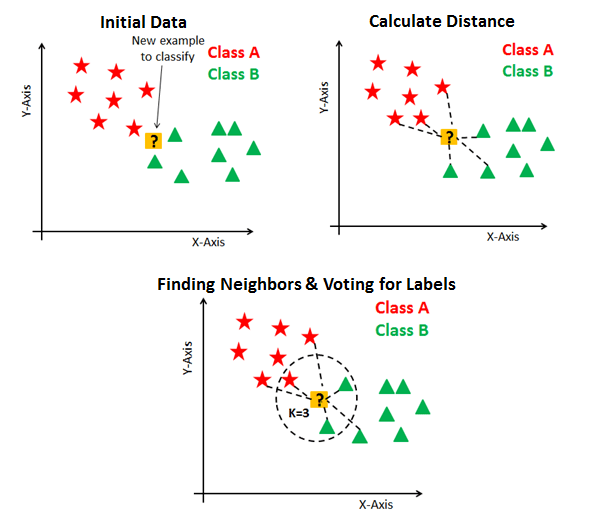
\includegraphics[scale=0.5]{./KNN_model.png}
\caption{KNN算法流程图解}
\label{fig:1}
\end{figure}

\subsubsection{算法细节}

KNN算法在实现时需要注意的细节如下

\begin{itemize}
	\item [-] 有时特征并不是量化的,譬如看两个词之间的关系,两个词均不是数字,此时无法直接利用KNN算法,因而需要先进行特征提取(feature extraction)和嵌入(embedding)。本例中,由于\verb|sklearn|中的数据已经进行了特征提取等,我们便无须再进行此步操作
	\item [-] 数据之间并不直接拥有“距离”,我们将不同种类的特征映射到线性空间的不同维度上,我们将映射后在线性空间中的点之间的位置的距离认作距离,是抽象出来的距离,常用欧式距离来进行计算,公式如下
	\begin{center}
		点$x_i(x^1_i,x^2_i,\ldots,x^l_i)$和$x_j(x^1_j,x^2_j,\ldots,x^l_j)$之间的距离\verb|Distance|满足:
	\end{center}
	\[\verb|Distance|=\sqrt{\sum_{k=1}^l{(x_k^i-x_k^j)^2}}\]
	\item [-] 由于k值会影响参与投票的点的数量,因而会极大程度地影响投票结果。所以需要调整k值找到最合适的k值以使预测结果尽可能精确。
\end{itemize}
\subsection{算法实现}
\subsubsection{模型初始化}
\begin{lstlisting}[style = python]
	def __init__(self, k=4):
        """Initialize the model with the given k value

        Args:
            k (int, optional): Defaults to 4.

        Raises:
            ValueError: k value must be a positive number
        """
        if k <= 0:
            raise ValueError("Invalid k value!It should be a positive number")
        self.k = k
        self.data = None
        self.label = None
\end{lstlisting}

\subsubsection{数据加载}
\begin{lstlisting}[style = python]
	def get_data(self, data, label):
        """This function is used to load the data

        Args:
            data (list): the feature of the dataset
            label (list): the label of the dataset
        """
        self.data = data
        self.label = label
\end{lstlisting}

\subsubsection{距离计算}
\begin{lstlisting}[style = python]
	@staticmethod
    def get_distance(point_1, point_2):
        differ_pow2 = [(point_1[i] - point_2[i]) ** 2 for i in range(len(point_1))]
        return math.sqrt(sum(differ_pow2))
\end{lstlisting}

\subsubsection{标签预测}
\begin{lstlisting}[style = python]
	def predict(self, point):
        """prediction the most probable label

        Args:
            point (list): the point to predict

        Returns:
            int : the label of the prediction
        """
        distance = dict()
        for i in range(len(self.data)):
            distance[i] = self.get_distance(self.data[i], point)			# 获取各点到预测点的距离
        sorted_index = [item[0] for item in sorted(distance.items(), key=lambda x: x[1])]	
        top_k_index = sorted_index[:self.k]									# 进行排序并获取前k个结果
        top_k = dict()
        label_set = set(self.label)
        for i in label_set:													# k个最近的邻点进行投票
            top_k[i] = 0
        for p in top_k_index:
            top_k[self.label[p]] += 1 
        top_k = sorted(top_k.items(), key=lambda x: -x[1])					# 找到票数最高的label作为预测值
        return top_k[0][0]
\end{lstlisting}

\subsubsection{正确率检测}
\begin{lstlisting}[style = python]
	def score(pred, labels):
    """count the accuracy based on the test dataset

    Args:
        pred (list): the prediction of the test dataset label
        labels (list): the true values of the test dataset label

    Returns:
        score (float): the score of the prediction
    """
    count = 0
    for i in range(len(pred)):
        if pred[i] == labels[i]:
            count += 1
    score = count / len(pred)
    return score
\end{lstlisting}

\subsection{实验结果}
\begin{itemize}
	\item [-] 由于\verb|iris|的样本数量较小,受随机化的影响很大,因而不同\verb|random.seed|结果大相径庭。
	\item [-] 样本数量小也导致简单交叉验证的比例影响也很大,因为参与训练的样本数量可能不够,准确性受影响。
	\item [-] k值的选取会直接影响参与投票的样本数量,因而需要寻找最合适的k值
\end{itemize}
	由此依据这几点进行实验,结果如下
\begin{figure}[!h]
\subfigure[random.seed=2019]
{
	\begin{minipage}[b]{.45\linewidth}
		\centering
		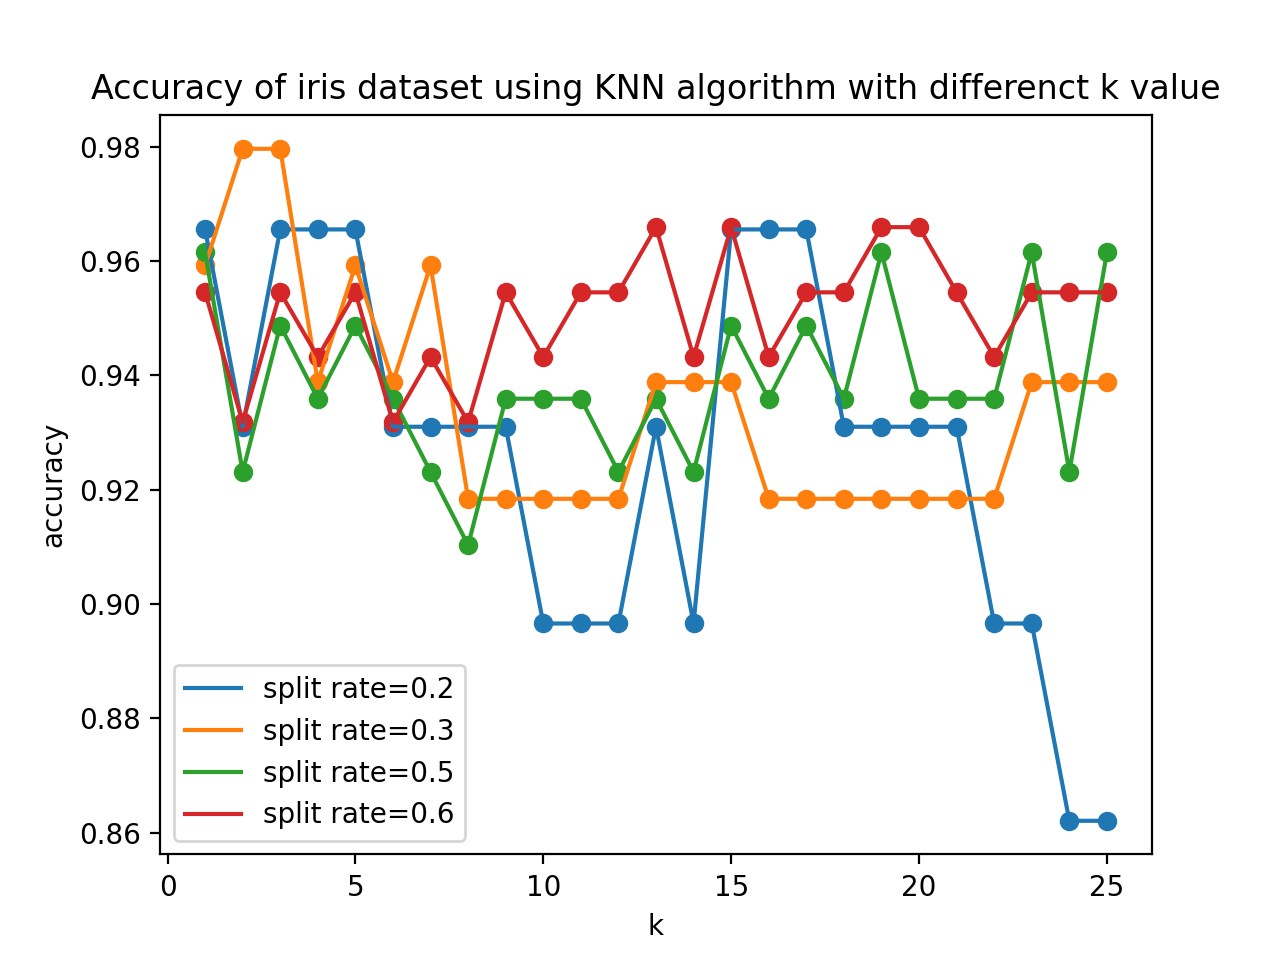
\includegraphics[width=\textwidth]{./result_seed_2019.png}
	\end{minipage}
}
\subfigure[random.seed=2021]
{
	\begin{minipage}[b]{.45\linewidth}
		\centering
		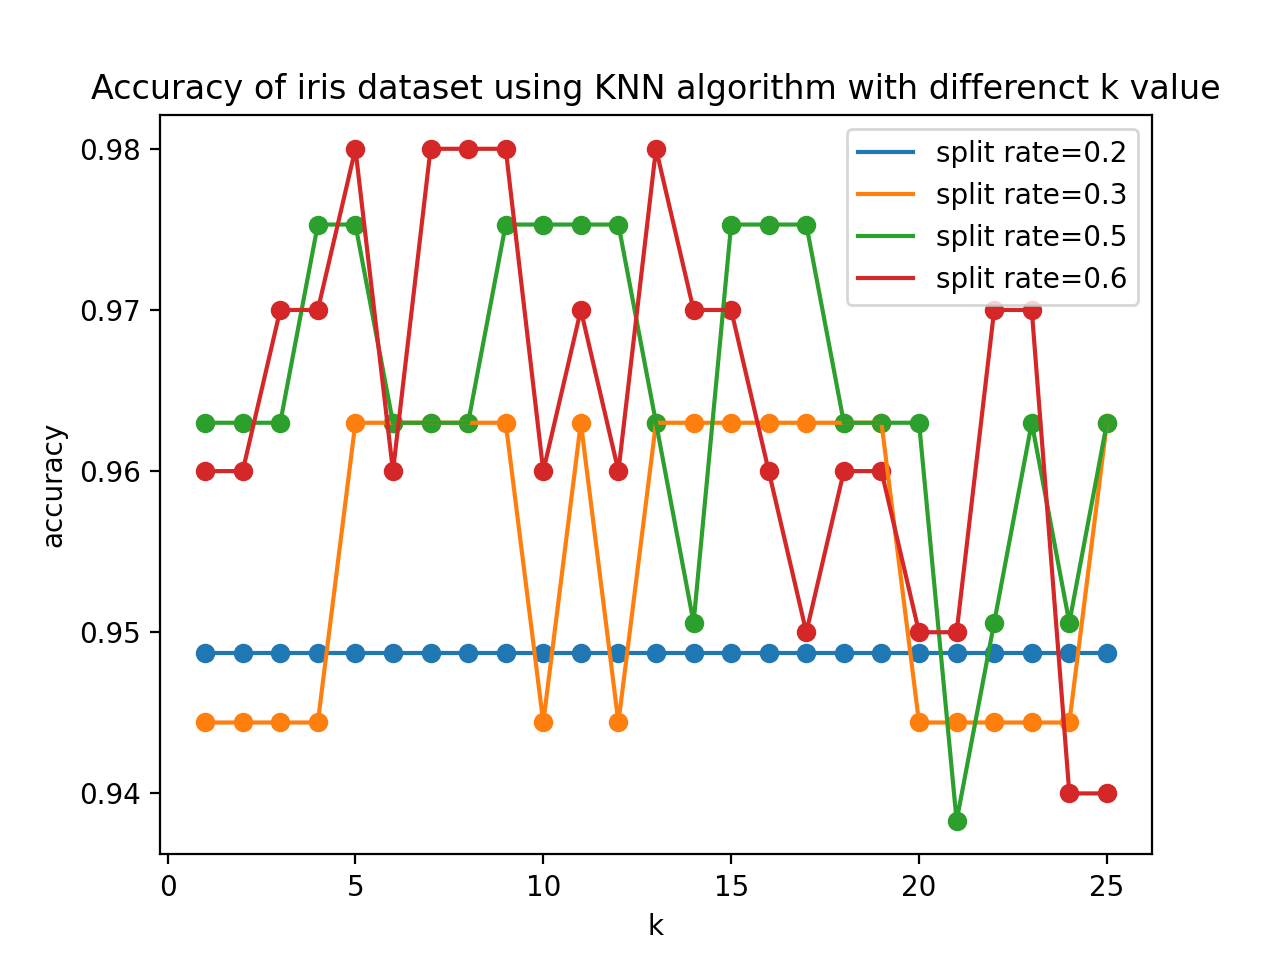
\includegraphics[width=\textwidth]{./result_seed_2021.png}
	\end{minipage}
}
\caption{实验结果}
\label{fig:2}
\end{figure}
\addtocounter{figure}{-1}
\begin{figure}[!h]
\addtocounter{subfigure}{2}
\centering
\subfigure[random.seed=810975]
{
	\begin{minipage}[b]{.45\linewidth}
		\centering
		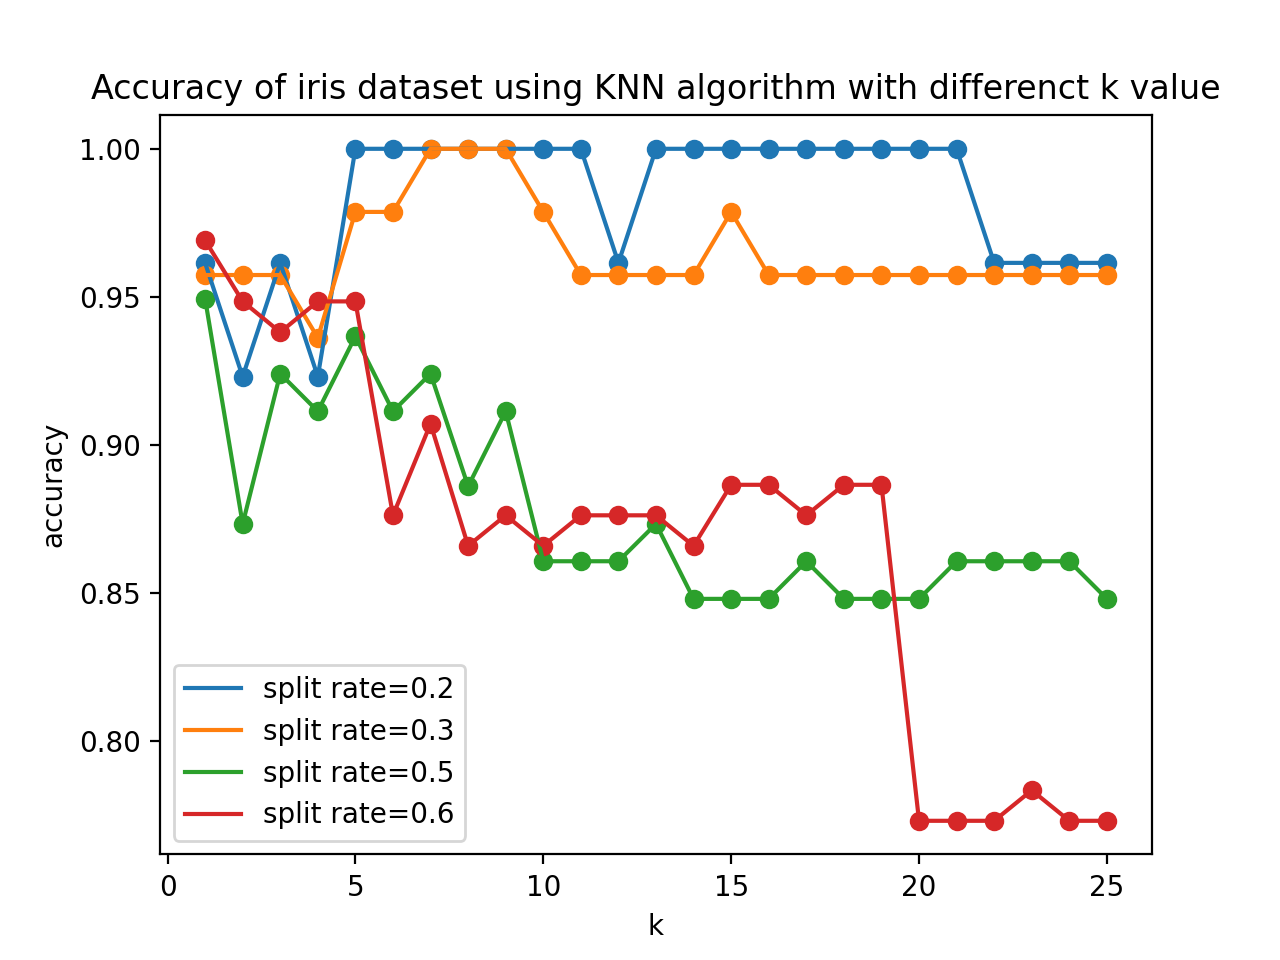
\includegraphics[width=\textwidth]{./result_seed_810975.png}
	\end{minipage}
}
\subfigure[random.seed=114514]
{
	\begin{minipage}[b]{.45\linewidth}
		\centering
		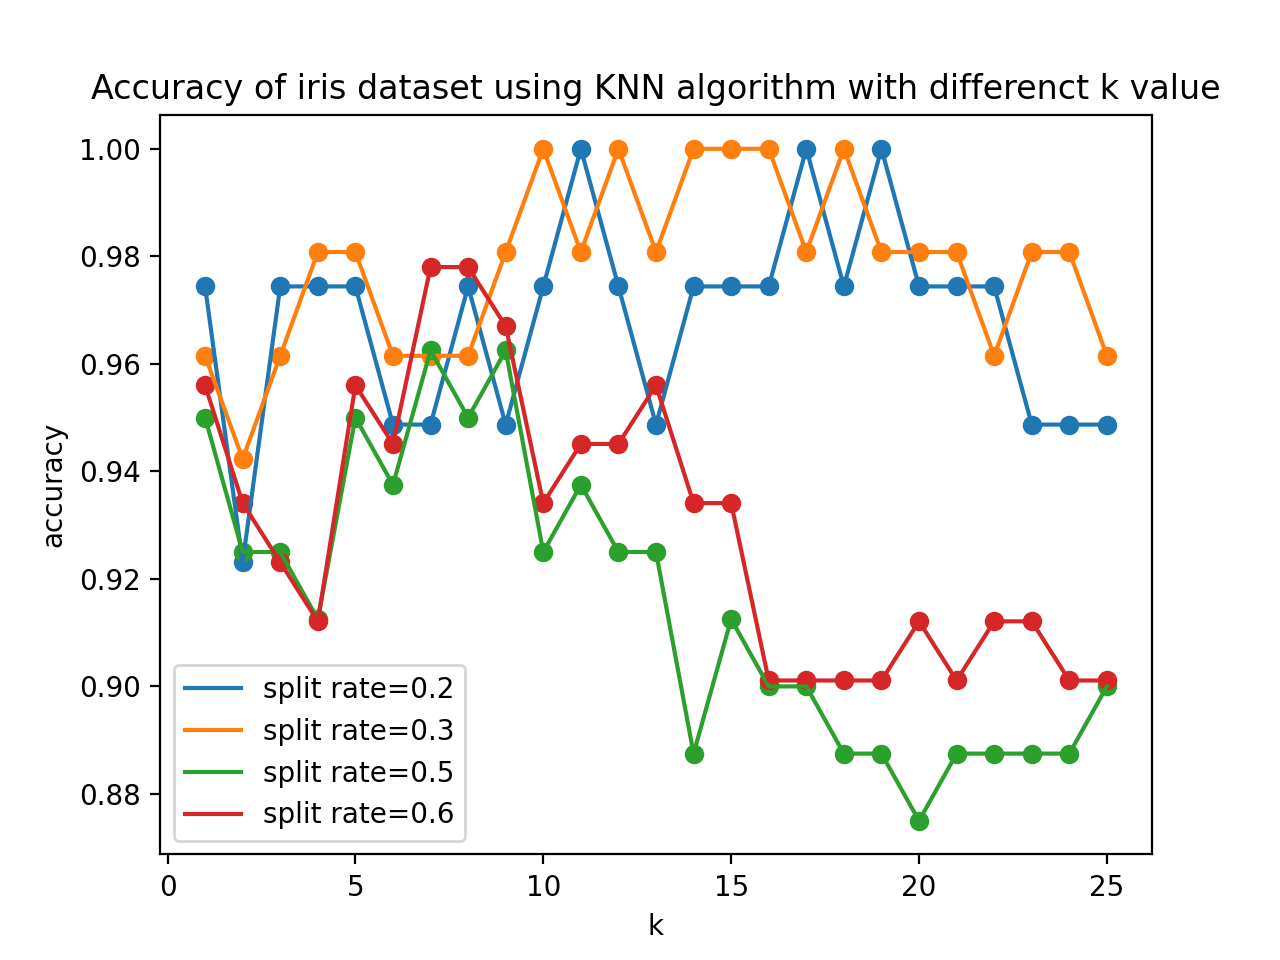
\includegraphics[width=\textwidth]{./result_seed_114514.png}
	\end{minipage}
}
\caption{实验结果}
\label{fig:2}
\end{figure}
\newpage

从实验结果可以发现由于数据量小,\verb|random.seed|对准确率分布的影响很大,但数据均有共同趋势,即为当k不断增大时,准确率会下降。这是因为k值较大时,参与投票的邻居太多,较后的邻居相关性较差,因而导致相关性下降。

\subsection{模型优化}

\subsubsection{优化思路}
\begin{itemize}
	\item [-] 鉴于数据量小,简单交叉验证中\verb|split_rate|对结果影响较大,为消除此影响,采用K折交叉验证,将数据等分成k组,然后每次用当中1组作为测试样本,其他组作为训练样本,每个组均进行相同操作,最后对准确率取平均。该方法同时可以避免\verb|random_seed|带来的影响。
	\item [-] 使用KD-Tree进行剪枝处理求k个最近邻居,但由于数据量只有150,因而认为使用KD-Tree会造成建树、剪枝时大量的资源浪费,因而放弃该优化思路。
	\item [-] 每个邻居的权重都相同,会导致可能出现两个标签票数相同的情况。而且,逻辑上而言更靠近预测点的邻居话语权应该更大、权重应该更大,因为投票时采用基于距离确定权重的方式,可以获得更准确的数据。
\end{itemize}

\subsubsection{优化结果}
自己未基于\verb|numpy|实现了一份KFold算法,使用了\verb|random.shuffle|以实现数据的乱序处理,代码如下
\begin{lstlisting}[style = python]
def _k_fold(data, label, k=10):
    """k fold algorithm to split the data

    Args:
		data (list): the raw dataset, it should be list or numpy.array
		label (type): the raw label dataset, it should be list or numpy.array
        k (int, optional): the total number of the groups. Defaults to 10.

    Returns:
        data_group_list, label_group_list : the list of the groups
    """
	if k <= 0:
		raise ValueError("Invalid k value!It should be a positive number")
    data_group_list = []                # to store the divided data groups
    label_group_list = []               # to store the divided label groups
    group_count = len(data)//k          # the number of data in a single group
    if type(data) == numpy.ndarray:
        data = data.tolist()            # turn the numpy.array into list
        label = label.tolist()          # otherwise the shuffle may go wrong
    data_copy = copy.deepcopy(data)
    label_copy = copy.deepcopy(label)
    random.seed(2021)
    random.shuffle(data_copy)
    random.seed(2021)
    random.shuffle(label_copy)
    for i in range(k):
        if i != k - 1:
            data_group = data_copy[i*group_count : (i+1)*group_count]
            label_group = label_copy[i*group_count : (i+1)*group_count]
        else:
            data_group = data_copy[i*group_count:]
            label_group = label_copy[i*group_count:]
        data_group_list.append(data_group)
        label_group_list.append(label_group)
    return data_group_list, label_group_list
\end{lstlisting}


完成\verb|KFold|算法后利用该算法进行交叉验证处理,重新进行了一次实验,实验结果如下

\begin{figure}[!h]
	\subfigure[devided into 10 groups]
	{
		\begin{minipage}[b]{.45\linewidth}
			\centering
			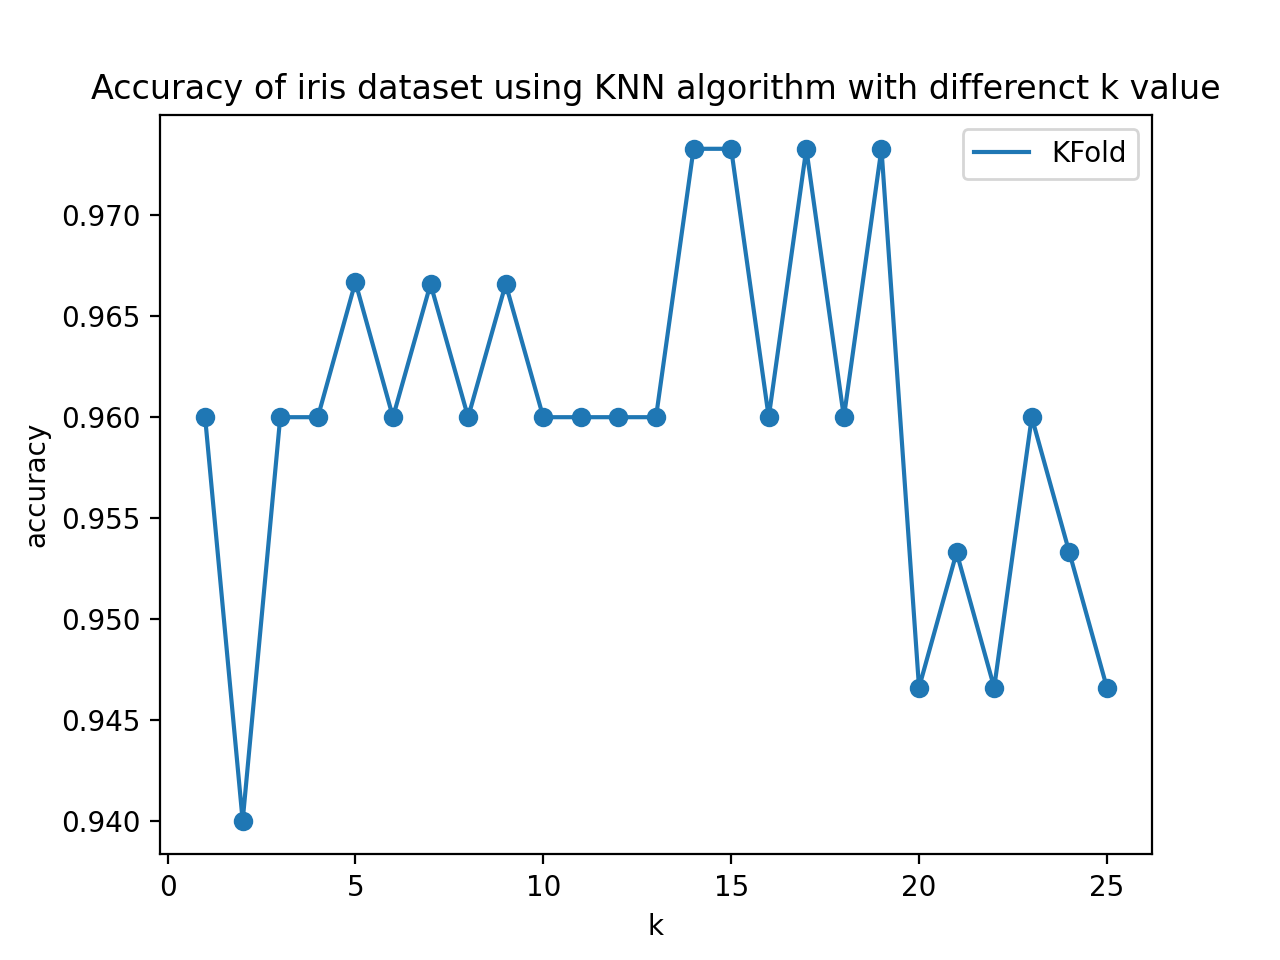
\includegraphics[width=\textwidth]{./k_fold_10.png}
		\end{minipage}
	}
	\subfigure[devided into 5 groups]
	{
		\begin{minipage}[b]{.45\linewidth}
			\centering
			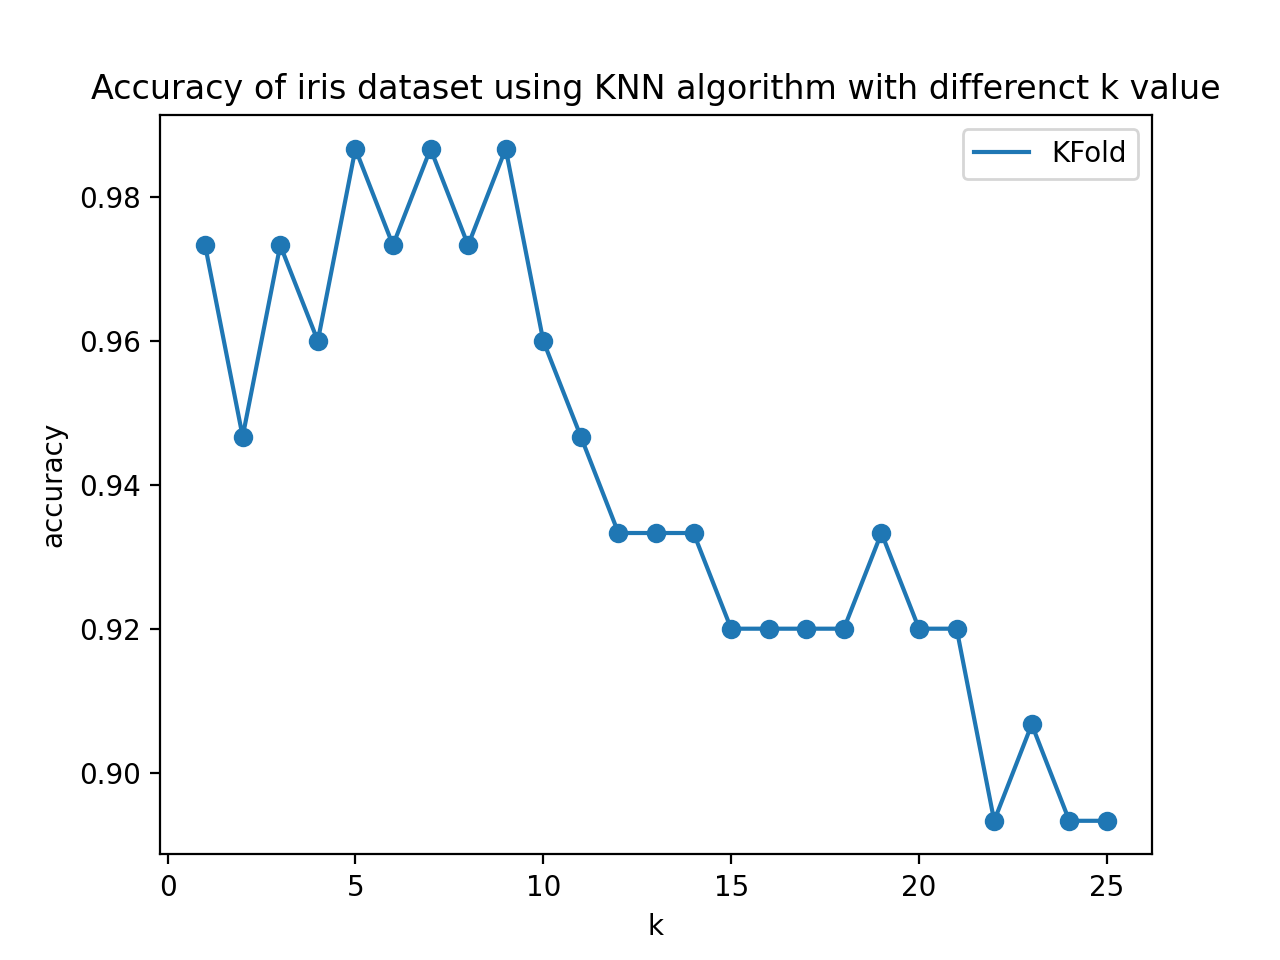
\includegraphics[width=\textwidth]{./k_fold_5.png}
		\end{minipage}
	}
	\caption{基于KFold算法的优化}
	\label{fig:2}
\end{figure}

再调整投票权重计算方式,调整方式(逻辑代码)和优化结果如下
\begin{lstlisting}[style = python]
	for neighbor in k_Nearest_Neighbors:
		_vote[neighbor.label] += constant_number / (distance(neighbor, point) + another_constant)
\end{lstlisting}

\begin{figure}[!h]
	\subfigure[random.seed=2019]
	{
		\begin{minipage}[b]{.45\linewidth}
			\centering
			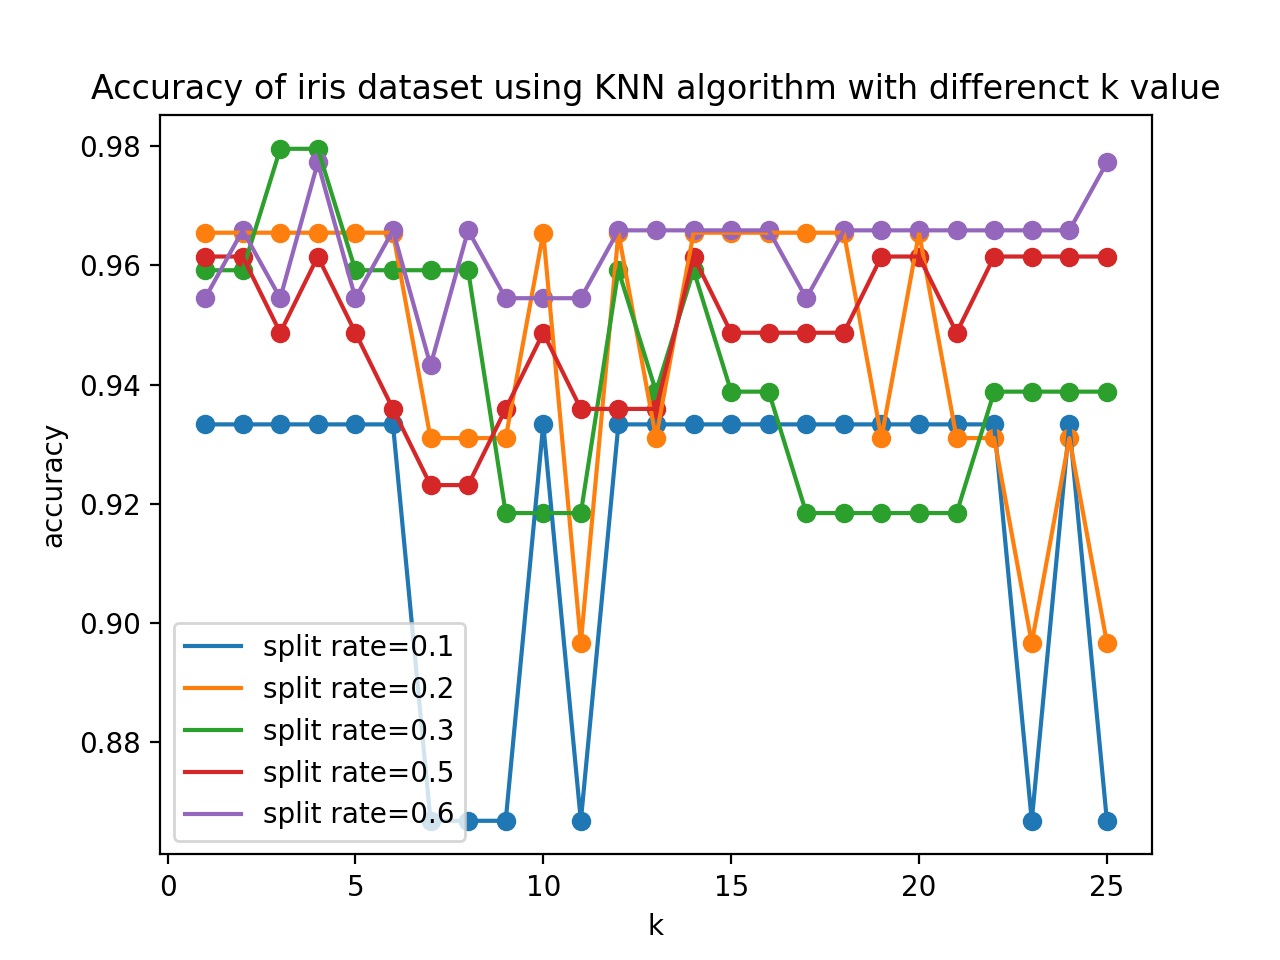
\includegraphics[width=\textwidth]{./weight_seed_2019.png}
		\end{minipage}
	}
	\subfigure[random.seed=2021]
	{
		\begin{minipage}[b]{.45\linewidth}
			\centering
			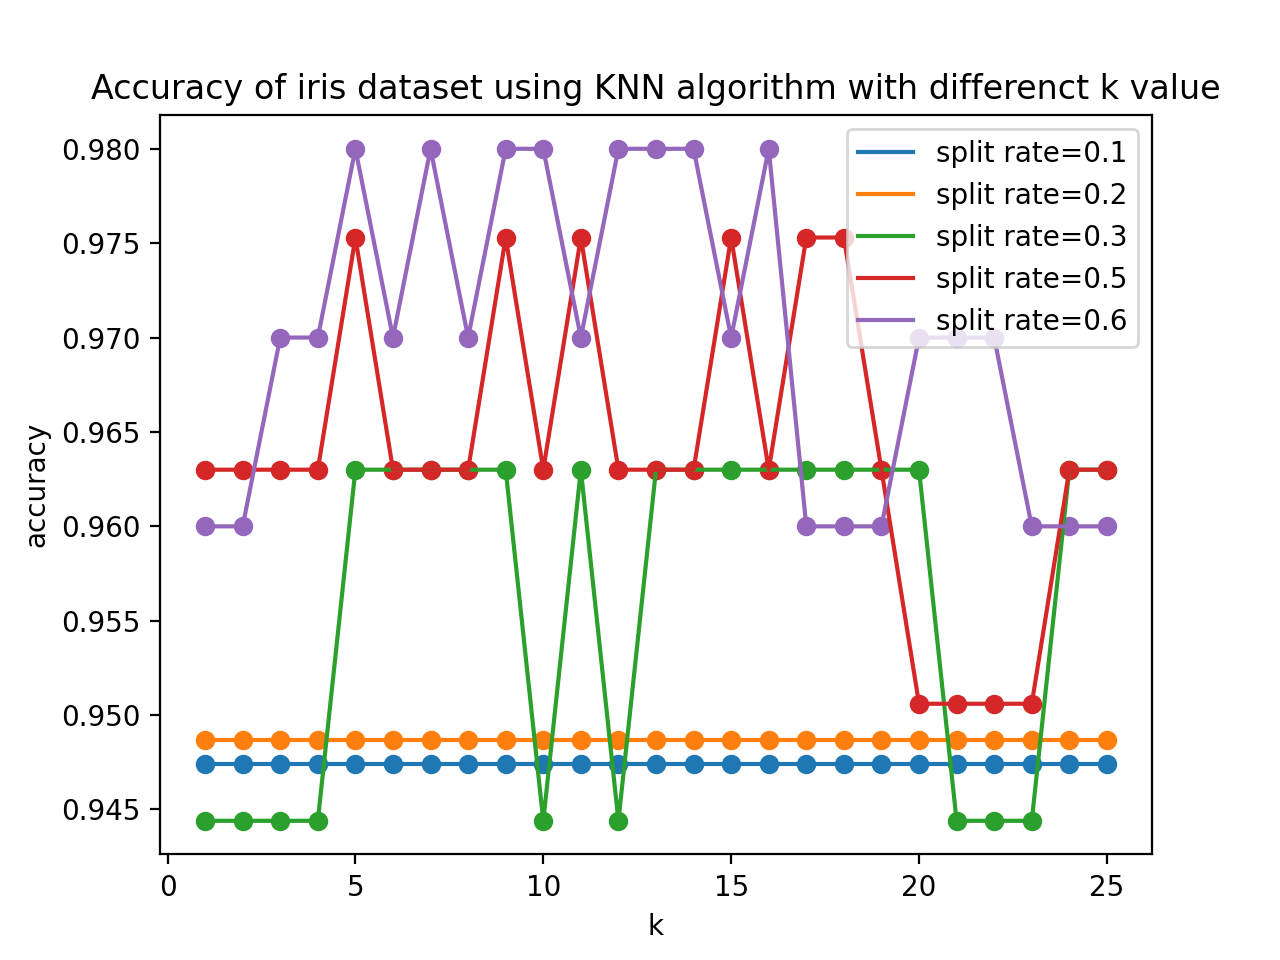
\includegraphics[width=\textwidth]{./weight_seed_2021.png}
		\end{minipage}
	}

\caption{基于权重策略调整的优化}
\label{fig:2}
\end{figure}
\addtocounter{figure}{-1}
\begin{figure}[!h]
\addtocounter{subfigure}{2}
\centering
	\subfigure[devided into 10 groups]
	{
		\begin{minipage}[b]{.45\linewidth}
			\centering
			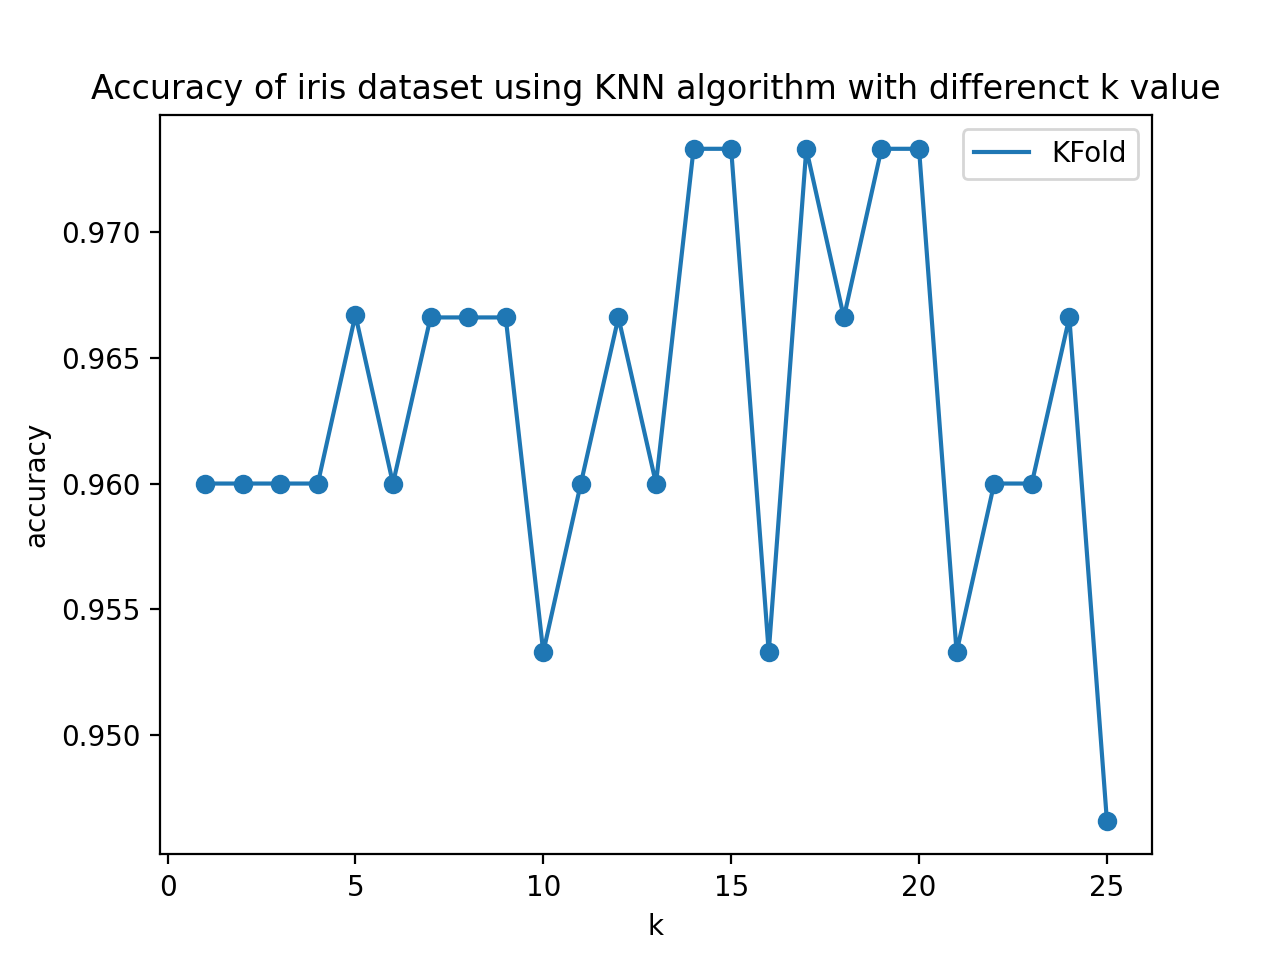
\includegraphics[width=\textwidth]{./weight_kfold_10.png}
		\end{minipage}
	}
	\subfigure[devided into 5 groups]
	{
		\begin{minipage}[b]{.45\linewidth}
			\centering
			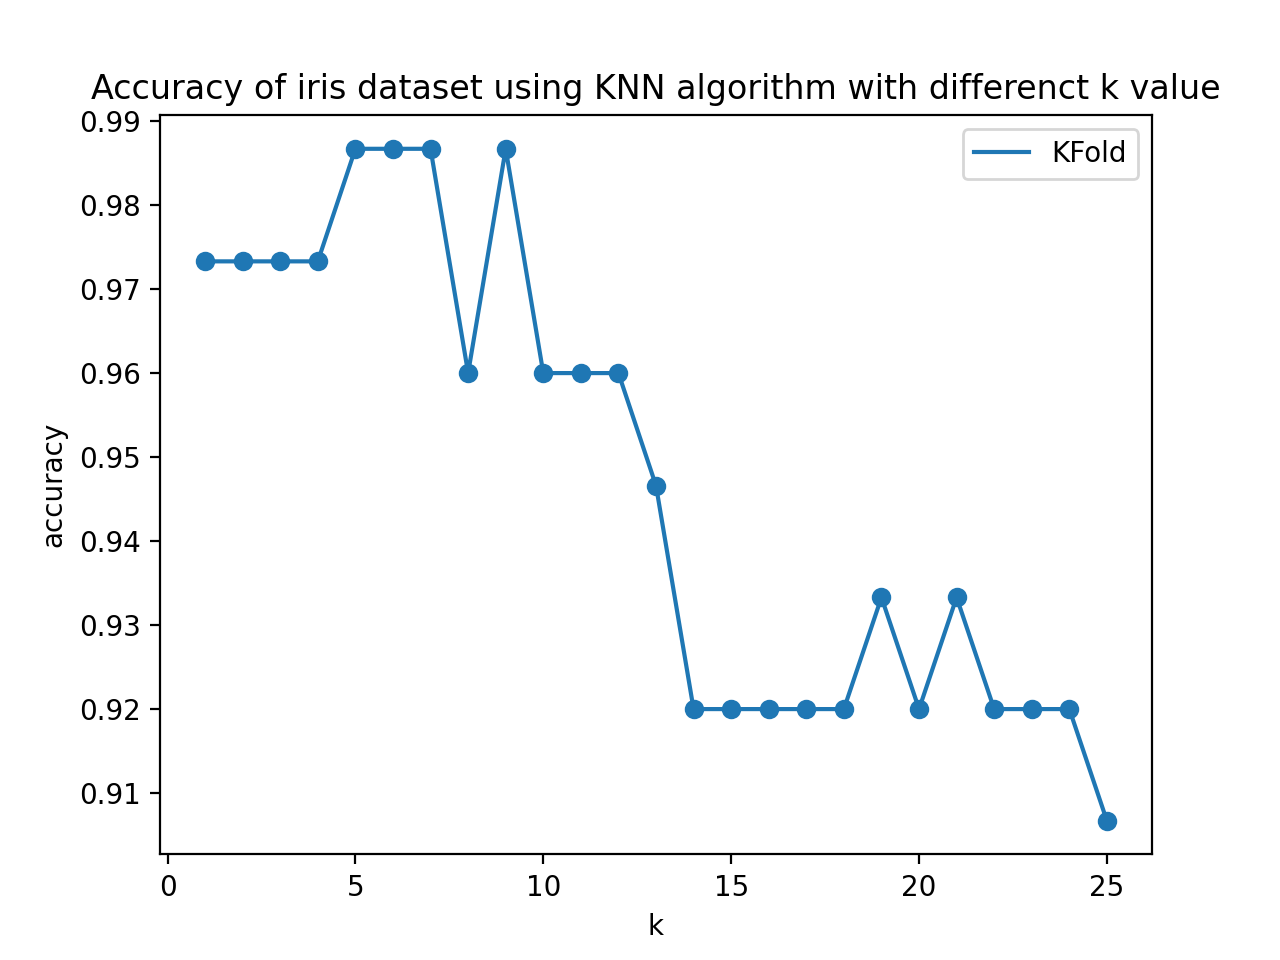
\includegraphics[width=\textwidth]{./weight_kfold_5.png}
		\end{minipage}
	}
	\caption{基于权重策略调整的优化}
	\label{fig:2}
\end{figure}

\newpage
从上述结果中可以得出,基于\verb|KFold|算法进行优化后,分成5组的情况比简单交叉验证时取\verb|split_rate=0.2|时更能体现准确率跟随k的变化的趋势,因而认为\verb|KFold|的优化是合理的。在对投票权重策略进行调整之后,准确率的变化更加平稳,且维持了较高水平,因而认为投票权重策略的优化也是合理的。。

\section{实验总结}
本次实验我通过纯Python实现了KNN算法,并使用简单交叉算法进行数据处理,并将结果进行可视化,得到了较好的结果,在k值取3-7之间有较好的效果,大概达到96\%左右。之后通过使用调整交叉验证算法,改用\verb|KFold|交叉验证算法进一步使得数据稳定,尽可能地利用到了各组数据;再通过调整投票权重策略使得结果更可信更有说服力。最终结果较好,但鉴于普通KNN已有很好的效果,优化并没有起到非常明显的效果,而且因为数据量较小,偶然因素影响较大,但逻辑上可知优化是合理且可行的。
\end{document}
